\chapter{Rapid and simultaneous estimation of fault slip and heterogeneous lithospheric viscosity from postseismic deformation}

\section{Summary}
Postseismic deformation is commonly attributed to viscoelastic
relaxation and/or afterslip, although discerning between the two
driving mechanisms can be difficult.  A major complication in modeling
postseismic deformation is that forward models can be computationally
expensive, making it difficult to adequately search model space to
find the optimal fault slip distribution and lithospheric viscosity
structure that can explain observable postseismic deformation.  We
propose an inverse method which uses coseismic and early postseismic
deformation to rapidly and simultaneously estimate a fault slip
history and an arbitrarily discretized viscosity structure of the
lithosphere. Our method is based on an approximation which is
applicable to the early postseismic period and expresses surface
deformation resulting from viscoelastic relaxation as a linearized
function with respect to lithospheric fluidity.  We demonstrate this
approximation using two-dimensional earthquake models.  We validate
the approximation and our inverse method using two three-dimensional
synthetic tests. The success of our synthetic tests suggests that our
method is capable of distinguishing the mechanisms driving early
postseismic deformation and recovering an effective viscosity
structure of the lithosphere.

\section{Introduction}
Geodetic observations of surface deformation in the months to years
following an earthquake are often attributed to afterslip
\citep[e.g.][]{Marone1991}, viscoelastic relaxation in the lithosphere
\citep[e.g.][]{Nur1974}, and/or poroelastic relaxation
\citep[e.g.][]{Peltzer1998}.  If postseismic deformation can be
entirely described by afterslip, then one could easily constrain the
spatial distribution of slip on prescribed fault geometries with a
linear least squares inversion \citep[e.g.][]{Harris1987,Burgmann2002,Freed2007},
which could then provide insight into the frictional properties of
faults \citep[e.g.][]{Hsu2006,Barbot2009}.  However, postseismic deformation
following large ($M_w\geq7$) earthquakes is often attributed to
viscoelastic relaxation in the lithosphere
\citep[e.g.][]{Hetland2003,Pollitz2003,Pollitz2005} or a combination of both afterslip
and viscoelastic relaxation \citep[e.g.][]{Freed2006a,Hearn2009,Johnson2009,Rollins2015}.
In such cases, postseismic deformation can be used to also constrain
the viscous properties of the lithosphere, although this is a more
difficult task than constraining just a slip distribution.  Not only
do the competing deformation mechanism need to be discerned, finding
the viscosity distribution of the lithosphere from postseismic
deformation is a computationally expensive nonlinear inverse problem.
Typically, the estimation of viscosities is approached with a forward
modeling, grid search or Monte Carlo method.  These forward modeling
techniques require the number of unknown parameters being estimated to
be small, meaning that significant and potentially inappropriate
modeling assumptions must be made.  Namely, studies seeking to
estimate the viscosity structure of the lithosphere often assume for
computational tractability that the lithosphere is composed of two or
three homogeneously viscoelastic layers, which may not be appropriate
for describing a more realistic depth dependent viscosity structure
\citep{Riva2009,Hines2013}.

In this paper we propose a relatively fast method to invert coseismic
and postseismic deformation to simultaneously estimate a
time-dependent distribution of fault slip and an arbitrarily
discretized viscosity structure of the lithosphere.  Our method is
based on an approximation which linearizes the rate of early
postseismic deformation with respect to the viscosity of the
lithosphere.  We demonstrate the effectiveness and limitations of our
method through two synthetic tests.

\section{Approximation for postseismic deformation} 
We assume that the lithosphere can be approximated as a Maxwell
viscoelastic material on the timescales of postseismic deformation,
where shear stress, $\mathbf{\sigma}$, and strain,
$\mathbf{\varepsilon}$, are related by
\begin{equation}
  \frac{\partial\mathbf{\varepsilon}}{\partial t}=\frac{\mathbf{\sigma}}{2\eta} + 
                              \frac{1}{2\mu}\frac{\partial\mathbf{\sigma}}{\partial t}.
\end{equation}
We use $\eta$ and $\mu$ to represent viscosity and shear modulus,
respectively.  This constitutive relationship implies that a sudden
strain from an earthquake will instantaneously stress the lithosphere
elastically (assuming the lithosphere is undergoing quasi-static
deformation).  Viscoelastic creep will initiate immediately after the
earthquake, where the initial viscous strain rate in each parcel of
the lithosphere will be proportional to the fluidity ($1/\eta$) in
that parcel, and independent of the fluidity elsewhere because the
initial stresses are only controlled by the elastic properties of the
lithosphere.  Stresses from the earthquake will dissipate over time
through viscoelastic relaxation.  During the period in which stress
changes from viscoelastic relaxation are small compared to the initial
elastic stresses, each parcel will continue to creep at a rate that is
approximately proportional to its fluidity.  In this early postseismic
period, the surface deformation from creep in each parcel will have an
amplitude that is also proportional to the fluidity in that parcel and
independent of the fluidity elsewhere.  As we will show, the early
surface expression of creep in the entire lithosphere is therefore a
sum of the surface deformation from each parcel and is linear with
respect to lithospheric fluidity.  We demonstrate this property of
early postseismic surface deformation in this section using simple
infinite length, strike-slip earthquake models, where the lithosphere
is approximated as a layered half-space. In Section \ref{SynthTest} we
consider two finite fault models with an arbitrarily discretized
lithospheric viscosity structure, the first with only Maxwell
viscoelasticity and the second with Burgers viscoelasticity.

\subsection{Two-dimensional earthquake models}\label{2DModel}
The easiest way to demonstrate how postseismic deformation can be
linearized with respect to lithospheric viscosity is with a
two-dimensional earthquake model consisting of a long, vertical,
surface rupturing, strike-slip fault that is embedded in a
viscoelastic horizontal layer overlying a viscoelastic half-space.  We
make use of the Correspondence Principle of Viscoelasticity
\citep[e.g.][]{Flugge1975}, which states that the Laplace transform of
deformation in a viscoelastic body has the same form as the Laplace
transform of deformation in a elastic body with the same geometry and
subjected to the same boundary conditions. The solution for
displacements following an earthquake in a viscoelastic lithosphere
can then be readily found provided that the corresponding elastic
solution is known \citep[e.g.][]{Nur1974,Savage1978,Hetland2005}.  One only
needs to replace the shear modulus in the Laplace transform of the
elastic solution with the effective viscoelastic shear modulus and
then compute the inverse Laplace transform.

\subsubsection{Two layered model}\label{2D2LModel}
From the solution of \citet{Rybicki1971}, surface displacements,
$u_{e}(x,t)$, resulting from slip on a fault in an elastic surface
layer overlying a semi-infinite elastic substrate are
\begin{equation}\label{TwoLayerElastic}
  u_{e}(x,t) = b(t)\left(\frac{1}{2} W(0) + 
    \sum_{n=1}^\infty \Gamma^nW(n)\right),
\end{equation}
where
\begin{equation}
  W(n) = \frac{1}{\pi}\left(\tan^{-1}\left(\frac{2nH + D}{x}\right) 
    - \tan^{-1}\left(\frac{2nH - D}{x}\right)\right)
\end{equation}
and
\begin{equation}
  \Gamma = \frac{\mu_1 - \mu_2}{\mu_1 + \mu_2}.
\end{equation}
In the above equation, $b(t)$ describes cumulative slip on the fault
through time and can describe coseismic slip and/or afterslip. $D$ is
the locking depth of the fault, $H$ is the thickness of the upper
layer, and $\mu_1$ and $\mu_2$ are the shear moduli in the upper
layer and lower substrate, respectively.  The Laplace transform of
eq. (\ref{TwoLayerElastic}) is
\begin{equation}\label{TwoLayerElasticLaplace}
 \hat{u}_e(x,s) = \hat{b}(s)\left(\frac{1}{2} W(0) +\sum_{n=1}^\infty\Gamma^nW(n)\right).
\end{equation}
We replace $\mu_1$ and $\mu_2$ in eq. (\ref{TwoLayerElasticLaplace})
with the equivalent shear moduli for Maxwell materials in the Laplace
domain, $\hat{\mu}_1$ and $\hat{\mu}_2$, to get the Laplace
transform of surface displacements in the two-layered, viscoelastic
half-space,
\begin{equation}\label{TwoLayerViscousLaplace}
 \hat{u}_v(x,s) = \hat{b}(s)\left(\frac{1}{2}W(0) +\sum_{n=1}^\infty\hat{\Gamma}^nW(n)\right),
\end{equation}
where
\begin{equation}
  \hat{\Gamma} = \frac{\hat{\mu_1} - \hat{\mu_2}}{\hat{\mu_1} + \hat{\mu_2}}
\end{equation}
and
\begin{equation}
  \hat{\mu_i} = \frac{s}{\frac{s}{\mu_i} + \frac{1}{\eta_i}}.
\end{equation}
To find the surface displacements in the time domain one must find the
inverse Laplace transform of eq. (\ref{TwoLayerViscousLaplace}), which
is typically done using the method of residues. However, we are
interested in characterizing the behavior of only the early
postseismic deformation and it serves us better to instead perform the
inverse Laplace transform with an extension of the initial value
theorem (Appendix A). We assume for simplicity that the shear modulus
for the viscoelastic lithosphere is homogeneous (i.e. $\mu_1 = \mu_2$)
and demonstrate in a supplementary IPython notebook that our
conclusions still hold when $\mu_1 \neq \mu_2$.  The surface
displacements in the time domain are
\begin{equation}
 u_v(x,t) = b(t)\frac{1}{2}W(0) + 
            b(t)\ast\mathcal{L}^{-1}\left[\sum_{n=1}^\infty\hat{\Gamma}^{n}W(n)\right],
\end{equation}
where we use $*$ to denote a convolution with respect to time.
Evaluating the above inverse Laplace transform using the method
described in Appendix A, we find
\begin{align}\label{TwoLayerViscous}
  u_v(x,t) = &b(t)\frac{1}{2}W(0) +\nonumber\\
             &b(t)\ast\left(\frac{\mu}{2\eta_2}W(1) - \frac{\mu}{2\eta_1}W(1)\right) +\nonumber\\
             &b(t)\ast\left(\left(\frac{\mu^2t}{4\eta_2^2} -
                  \frac{\mu^2t}{4\eta_1\eta_2}\right) \left(W(1) - W(2)\right) +
                  \left(\frac{\mu^2t}{4\eta_1\eta_2} - \frac{\mu^2t}{4\eta_1^2}\right)
                  \left(W(1) + W(2)\right)\right) + \nonumber\\ 
             &\dots.
\end{align}
The first term in eq. (\ref{TwoLayerViscous}) is the elastic response
to slip on the fault.  The remaining terms describe the surface
displacement due to viscoelastic relaxation.  We refer to the first of
these remaining terms as the initial viscoelastic response, which
describes surface deformation resulting from viscoelastic creep during
the period in which the stresses from fault slip are unaltered by
viscoelastic relaxation.  The initial viscoelastic response is linear
with respect to the fluidity in each of the two layers.

If the time since the rupture is sufficiently small compared to the
relaxation times of each layer, $\tau_i=\eta_i/\mu$, (i.e. the third
and following terms in eq. (\ref{TwoLayerViscous}) are small) and the
timescale of slip described by $b(t)$ is also short compared to the
relaxation times in the half-space, then we can truncate the series and
approximate early surface deformation using only the elastic response
and the initial viscoelastic response,
\begin{equation}\label{TwoLayerViscousApprox}
 u_v(x,t) \approx b(t)\frac{1}{2}W(0) + 
          \int_0^t b(\theta)\left(\frac{\mu}{2\eta_2}W(1) - 
                  \frac{\mu}{2\eta_1}W(1)\right)d\theta.
\end{equation} 
An approximation similar to eq. (\ref{TwoLayerViscousApprox}) was
demonstrated by \citet{Segall2010} for an elastic layer over a Maxwell
viscoelastic substrate. 

\begin{figure}\label{figure1}
  \centering 
  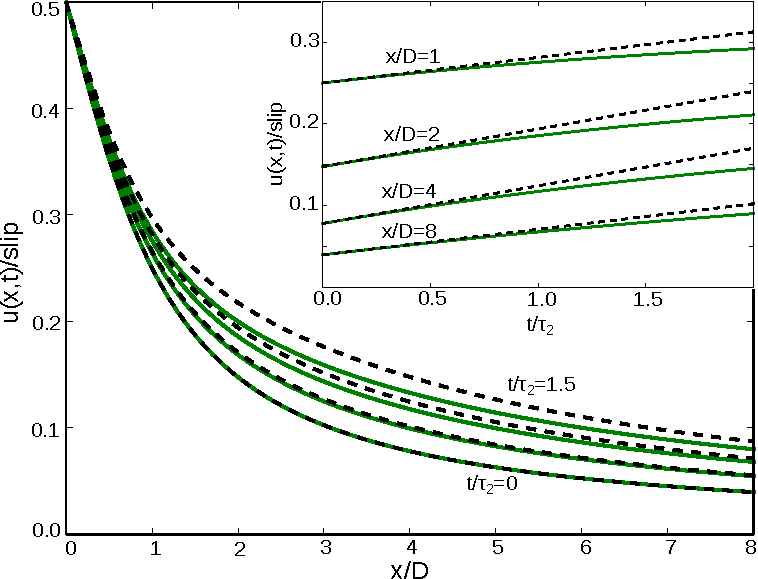
\includegraphics{ch2/figures/Fig1.pdf}
  \caption{Surface displacements predicted by
    eq. (\ref{TwoLayerViscous}) truncated after ten terms (green) and
    the approximation given by eq. (\ref{TwoLayerViscousApprox})
    (dotted black).  Times are normalized by the lowest relaxation
    time in the lithosphere, $\tau_2$, and distances are normalized by
    the fault locking depth, $D$.  Displacements are shown as a
    function of distance from the fault at times $t/\tau_2 =
    0.0,0.5,1.0$ and $1.5$. The inset figure shows displacement time
    series at locations $x/D = 1, 2, 4$ and $8$.}
  \label{Figure 1}
\end{figure} 

Fig. 1 shows the series solution from eq. (\ref{TwoLayerViscous})
truncated after sufficiently many terms along with the approximation
given by eq. (\ref{TwoLayerViscousApprox}). In this comparison, we use
$H=15$ km, $D=10$ km and a shear modulus of 32 GPa throughout the
lithosphere.  The upper layer is given a viscosity of $10^{20}$ Pa s
($\tau\approx 100$ years) and the substrate is given a viscosity of
$10^{19}$ Pa s ($\tau\approx 10$ years).  We let $b(t)$ describe a
unit of instantaneous slip at $t=0$.  In the series solution, the
rate of surface deformation decreases over time as stresses in the
half-space decay through viscoelastic relaxation.  Because $b(t)$ is a
constant after $t=0$, the initial viscoelastic response in
eq. (\ref{TwoLayerViscousApprox}) describes a constant rate of surface
deformation and so eq. (\ref{TwoLayerViscousApprox}) is a good
approximation for as long as the rate of deformation predicted by
eq. (\ref{TwoLayerViscous}) is also approximately constant. We find
the that the approximation is indistinguishable from the series
solution for at least as long as half the lowest of the two relaxation
times, regardless of our choice of model parameters.  The
approximation breaks down faster than what is show in Fig. 1 when
the upper layer is more fluid than the substrate or when we decrease the
depth of the material interface (i.e. when the more fluid material is
closer to the fault).  We also note that the approximation has more
longevity for locations further away from the fault, where it starts
to break down at about the minimum relaxation time in the lithosphere.

\subsubsection{Three layered and continuous depth dependent models}\label{2d3LModel}
We follow the same procedure as above to find the surface
deformation resulting from slip on a strike-slip fault in a three
layered viscoelastic half-space.  Starting from the layered elastic
solution from \citet{Chinnery1972}, we evaluate the solution for the
viscoelastic problem in our supplementary IPython notebook.  We find
the initial viscoelastic response to a unit of slip to be
\begin{equation}\label{ThreeLayerViscousResponse}
\frac{\partial}{\partial t}u(x,t)\big|_{t=0} = \frac{\mu}{2\eta_3}W(1,1)
                                      +\frac{\mu}{2\eta_2}(W(0,1) - W(1,1))
                                      -\frac{\mu}{2\eta_1}W(0,1),
\end{equation}
where
\begin{equation}
  W(n,m) = \frac{1}{\pi}\left(\tan^{-1}\left(\frac{2nH_2 + 2mH_1 + D}{x}\right) - 
                              \tan^{-1}\left(\frac{2nH_2 + 2mH_1 - D}{x}\right)\right),
\end{equation}
$\eta_1$, $\eta_2$, and $\eta_3$ are the viscosities of the top,
middle, and bottom layers, respectively, and $H_1$ and $H_2$ are the
thicknesses of the top and middle layers, respectively.  We see that
eq. (\ref{ThreeLayerViscousResponse}) is once again linear with
respect to the fluidity in each of the three layers.  We can
approximate early postseismic deformation resulting from slip
described by $b(t)$ as
\begin{equation}\label{ThreeLayerViscousApprox}
u(x,t) \approx b(t)\frac{1}{2} W(0,0) + 
         \int_0^tb(\theta)\left(\frac{\mu}{2\eta_3}W(1,1)
                               +\frac{\mu}{2\eta_2}(W(0,1) - W(1,1))
                               -\frac{\mu}{2\eta_1}W(0,1)\right)d\theta.
\end{equation}
We can see that eq. (\ref{ThreeLayerViscousApprox}) reduces to eq.
(\ref{TwoLayerViscousApprox}) when $\eta_3 = \eta_2$.

At this point we posit that a similar approximation can be made for an
arbitrarily layered lithosphere. In Appendix B we use
eq. (\ref{ThreeLayerViscousResponse}) to find an initial viscoelastic
response kernel.  We then integrate that kernel over the depth of the
lithosphere to find the initial viscoelastic response for an arbitrary
depth dependent viscosity structure.  If the lithosphere is elastic
above the fault depth, $D$, and described by $\eta(z)$ below $D$ then
early postseismic deformation can be approximated as
\begin{equation}\label{ContinuousViscousApprox}
u(x,t) \approx \frac{b(t)}{\pi}\tan^{-1}(\frac{D}{x}) + 
               \int_o^t\int_D^\infty \frac{\mu b(\theta)}{2\pi\eta(z)}
                                    \left(\frac{2x}{x^2 + \left(D + 2z\right)^2} - 
                                    \frac{2x}{x^2 + \left(2z - D\right)^2}\right)
                                    dz d\theta.
\end{equation}
Although the above equation is capable of describing surface
deformation for an arbitrary depth dependent viscosity structure, it
falls short of being useful as the forward solution in an inverse
problem aimed at estimating lithospheric viscosity.  This shortcoming
is because the above equation makes the nonphysical assumption that the
fault is infinitely long, in addition to the restriction of only being
applicable to a vertical strike-slip fault.  The assumption of
infinite length would introduce first order errors, which would likely
wash out the second order effect of viscosity. However,
eq. (\ref{ContinuousViscousApprox}) is useful for making estimates of
the depth sensitivity of postseismic deformation.

\subsection{Three-dimensional earthquake models}\label{3DModel}
Motivated by our above results, we make the assertion that the initial
viscoelastic response to an instantaneous unit dislocation in a
three-dimensional Maxwell viscoelastic medium, which has been
arbitrarily discretized into $N$ regions, will have the form
\begin{equation}\label{PostseismicInitialVelocity}
  \frac{\partial}{\partial t}\vec{u}(\vec{x},t)\big|_{t=0} = \sum_j^N\frac{1}{\eta_j}G_j(\vec{x}).
\end{equation}
We denote $\vec{u}$ and $\vec{x}$ as vectors to emphasize that
eq. (\ref{PostseismicInitialVelocity}) is generalized to
three-dimensional problems.  We use $G_j(\vec{x})$ to represent the
initial rate of surface deformation at position $\vec{x}$ resulting
from viscoelastic creep in region $j$ with unit fluidity, where
fluidity is zero (i.e. elastic) in all other regions.  In this sense,
$G_j(\vec{x})$ can be thought of as a Green's function for the initial
viscoelastic response, and thus we refer to $G_j(\vec{x})$ as the initial
viscoelastic Green's functions.  We verify
eq. (\ref{PostseismicInitialVelocity}) numerically in Section \ref{Validation} and
save a theoretical justification for a later paper.

Using eq. (\ref{PostseismicInitialVelocity}), we can approximate
early surface deformation in a form that is consistent with
eqs. (\ref{TwoLayerViscousApprox}) and
(\ref{ThreeLayerViscousApprox}):
\begin{equation}\label{intermediate}
\vec{u}(\vec{x},t) \approx b(t)F(\vec{x}) + \sum_j^N\int_0^t
\frac{b(\theta)}{\eta_j}G_j(\vec{x}) d\theta,
\end{equation}
where $F(\vec{x})$ is the elastic Green's function, which describes the
elastic deformation resulting from a dislocation.  We further
generalize the approximation of surface deformation in
eq. (\ref{intermediate}) to allow for an arbitrary spatial
distribution of slip by using linear superposition.  If the elastic
deformation in a viscoelastic lithosphere can be described in terms of
$M$ elastic dislocation sources, then early surface deformation
resulting from both elastic dislocations and viscous creep can be
approximated as 
\begin{equation}\label{Postseismic_Approximation}
\vec{u}(\vec{x},t) \approx \sum_i^Mb_i(t)F_i(\vec{x}) +
\sum_i^M\sum_j^N\int_0^t\frac{b_i(\theta)}{\eta_j}G_{ij}(\vec{x}) d\theta.
\end{equation}
The initial viscoelastic Green's function is dependent upon both the
region it represents as well as the dislocation source inducing the
viscoelastic creep in that region, hence the two indices on
$G_{ij}(\vec{x})$.  It is worth restating that the approximation given
above does not account for the viscoelastic coupling between the
regions, since in eq. (\ref{Postseismic_Approximation}) each region's
contribution to surface deformation is independent of the viscosity
elsewhere.  This approximation is therefore appropriate for as long as
the regions do not significantly transfer stresses between each other
through viscoelastic deformation.  Alternatively, since our initial
viscoelastic Green's functions do not have time dependence, one could
view eq. (\ref{Postseismic_Approximation}) as being appropriate up
until surface velocities resulting from viscoelastic creep have
decayed appreciably.

\section{Inversion method}\label{InverseMethod}
The approximation of postseismic deformation given by eq.
(\ref{Postseismic_Approximation}) can be cast as an inverse problem
aimed at finding the distribution of slip on a fault and an
arbitrarily complicated lithosphere viscosity structure from
postseismic deformation. We assume that the slip history in any one
direction on each fault patch, $b_i(t)$, can be expressed as $P$ linear
terms such that
\begin{equation}
  b_i(t) = \sum_k^P \alpha_{ik}A_k(t),
\end{equation}
where $A_k(t)$ can be any parameterized slip function.  For this
paper $A_k(t)$ consists of either unit step functions describing
coseismic slip on a fault patch, or ramp functions, which increase
from 0 to 1 over some time interval, that are intended to represent
afterslip.  The coefficient $\alpha_{ik}$ then represents either the
amount of coseismic slip or the cumulative slip over a time interval.
The approximation given by eq. (\ref{Postseismic_Approximation}) now
becomes
\begin{equation}\label{Postseismic_Approximation2}
  \vec{u}(\vec{x},t) \approx
  \sum_i^M\sum_k^P\alpha_{ik}F_i(\vec{x})A_k(t) +
  \sum_i^M\sum_j^N\sum_k^P\int_0^t\frac{\alpha_{ik}}{\eta_j}G_{ij}(\vec{x})A_k(\theta)d\theta.
\end{equation}
If we assume a fault geometry and the elastic properties of the
lithosphere, $F_i(\vec{x})$ can be computed with finite element
software or with an analytic solution, for instance using
\citet{Okada1992} or \citet{Meade2007}. Likewise, $G_{ij}(\vec{x})$ can be
computed using finite element software.  If the assumed geometry of
the viscoelastic regions is sufficiently simple, $G_{ij}(\vec{x})$ may
also be computed with semi-analytic techniques
\citep[e.g.][]{Pollitz1997,Fukahata2006,Barbot2010}.

We estimate the unknown slip parameters, $\alpha_{ik}$, and unknown
viscosities in each region of the lithosphere, $\eta_j$, from
observations of surface deformation in a least squares sense. Let
$\mathbf{u_{\mathrm{obs}}}$ be a vector of observed coseismic and
postseismic surface displacements at various locations and points in
time.  Let $\mathbf{m}$ be a vector of all the unknown parameters
$\alpha_{ik}$ and $\eta_j$, and let $\mathbf{u(m)}$ be a vector of
postseismic surface displacements predicted by eq.
(\ref{Postseismic_Approximation2}). We seek to solve
\begin{equation}\label{Inverse_Problem}
  \mathrm{min}
  \big|\big|\mathbf{f(m)}\big|\big|_2^2
\end{equation}
subject to the constraint that
\begin{equation}
  \mathbf{m}\geq0,
\end{equation}
where 
\begin{equation}\label{ResidualFunction}
  \mathbf{f(m)} = 
    \begin{vmatrix}
      \mathbf{W\left(u(m)-u_{\mathrm{obs}}\right)}\\
      \lambda_s\mathbf{L_sm}\\
      \lambda_v\mathbf{L_vm}\\
    \end{vmatrix} .
\end{equation}  
In the above equation, $\mathbf{W}$ is a diagonal matrix containing the
reciprocal of the data uncertainties
(i.e. $\mathbf{W^TW}=\mathbf{C_d^{-1}}$ where $\mathbf{C_d}$ is
the data covariance matrix), and $\mathbf{L_s}$ and $\mathbf{L_v}$ are
regularization matrices.

We impose a non-negativity constraint on $\mathbf{m}$ which ensures that
inferred slip is in one predominant direction and that viscosities are
positive.  Specifically, the rake of the inferred slip on each fault
patch is constrained to be within a $90^\circ$ window defined by the
rakes of chosen orthogonal basis slip directions. For instance, the
basis slip directions could be chosen such that only slip rakes within
$45^\circ$ of pure strike-slip, normal, or thrust are permissible.

Because this inverse problem inevitably has non-unique solutions for
$\mathbf{m}$, we put additional constraints on the inferred slip and
inferred viscosity with the matrices $\mathbf{L_s}$ and $\mathbf{L_v}$,
respectively.  In our following synthetic test, we constrain the
solution by minimizing the Laplacian of the spatial distribution of
fault slip and lithospheric viscosity by letting $\mathbf{L_s}$ and
$\mathbf{L_v}$ be umbrella operators \citep{Desbrun1999}.  The parameters
$\lambda_v$ and $\lambda_s$ in eq. (23) control how much we enforce
the smoothness constraint.  In our synthetic test, we choose these
parameters using L-curves, which describe the trade off between the
model smoothness and data misfit.  We first set $\lambda_v=0$ and then
use an L-curve to pick $\lambda_s$.  We then fix $\lambda_s$ at our
chosen value and use another L-curve to pick $\lambda_v$.  We explored
using cross-validation to choose our model parameters, but we found
that the optimal pair of penalty parameters picked through
cross-validation tended to significantly degrade our fit to near-field
sites.

We find $\mathbf{m}$ that satisfies the above conditions using the
Gauss-Newton method \citep[e.g.][]{Aster2011}.  The best fit model parameters are
found by making an initial guess for the solution and then iteratively
solving
\begin{equation}\label{Gauss-Newton}
\mathbf{J}(\mathbf{m}^{k})\mathbf{m}^{k+1} = -\mathbf{f}(\mathbf{m}^k) + \mathbf{J}(\mathbf{m}^{k})\mathbf{m}^{k}
\end{equation}
for $\mathbf{m}^{k+1}$, where $\mathbf{J}(\mathbf{m}^k)$ is the Jacobian
of $\mathbf{f(m)}$ with respect to $\mathbf{m}$ evaluated at
$\mathbf{m^k}$. We impose the non-negativity constraint on $\mathbf{m}$
by solving eq. (\ref{Gauss-Newton}) with a non-negative least squares
algorithm \citep{Lawson1995}. In a nonlinear least squares algorithm,
computing the Jacobian can often be the largest computational burden
when an analytic solution for the Jacobian is not available. By
linearizing the viscoelastic response in early postseismic deformation
with respect to $1/\eta_j$, we have made our forward problem,
eq. (\ref{Postseismic_Approximation2}), sufficiently simple that
evaluating its Jacobian for a given $\mathbf{m}$ only requires a few
computationally inexpensive matrix operations. Consequently, our
nonlinear least squares algorithm converges to a solution for
$\mathbf{m}$ in a matter of seconds on a desktop computer.  The main
computational burden is in computing $F_i(x)$ and $G_{ij}(x)$ which
only needs to be done once for a given fault and lithosphere geometry.

\begin{figure}\label{figure2}
  \centering
  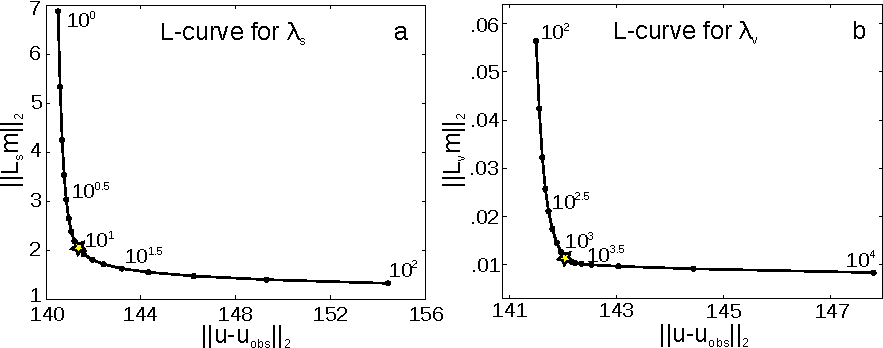
\includegraphics{ch2/figures/Fig2.pdf}
  \caption{L-curves used to select the penalty parameters. Panel (a)
    shows the trade-off between slip smoothness and data misfit while
    varying $\lambda_s$ and keeping $\lambda_v$ fixed at zero.  Panel
    (b) shows the trade off between smoothness of inferred viscosity and
    misfit while varying $\lambda_v$ and keeping $\lambda_s$ fixed at
    the value chosen from Panel (a).  Stars indicate our chosen penalty
    parameters.}
  \label{Figure 2}
\end{figure}

\section{Synthetic test}\label{SynthTest}
We demonstrate with two synthetic tests that our inverse method is
capable of recovering fault slip and an effective lithospheric
viscosity from postseismic deformation.  We use the finite element
software, PyLith \citep{Aagaard2013}, to compute the surface deformation
resulting from a specified amount of slip on a fault in a lithosphere
with either Maxwell or Burgers viscoelasticity.  We invert this
synthetic surface deformation using the method described above to
recover the imposed model parameters.  The synthetic tests also serve
to demonstrate that eqs. (\ref{PostseismicInitialVelocity}) and
(\ref{Postseismic_Approximation}) are indeed valid for three
dimensional earthquake models.

Our synthetic models consist of a 50 km long by 20 km wide strike-slip
fault, striking to the north and dipping $60^{\circ}$ to the east
(Fig. 5). At $t=0$ we impose $6.5\times 10^{19}$ N m of surface
rupturing, right-lateral coseismic slip with a distribution shown in
Fig. 3. After the coseismic slip, we impose 2 years of afterslip just
below the coseismic rupture zone.  The spatial distribution of
afterslip on the fault remains constant throughout the 2 years but the
rate of afterslip decreases by a factor of 2 every 0.5 years.  The
cumulative moment of afterslip over the first year is about $1.6\times
10^{19}$ N m, while the cumulative moment of afterslip over the second
year is $4.0\times 10^{18}$ N m.  We do not impose any fault slip
beyond $t=2$ years.

We compute surface displacements at 50 randomly chosen observation
points within a 400 km square centered about the fault (Fig. 5), which
is intended to roughly correspond with the density of GPS station at a
well instrumented plate boundary.  Displacements are computed at 0.05
year intervals up until $t=10$ years.  We add temporally correlated
noise to the computed displacements through time, consistent with what
one would expect from GPS observations.  The standard deviation of
northing and easting displacements is 1 mm, and the standard deviation
of the vertical displacements is 2.5 mm.  We add temporal covariance
with an exponential noise model that has a characteristic timescale of
0.25 years, which is intended to simulate seasonal processes that are
typically present in GPS time series.

\subsection{Green's functions}\label{GreensFunc}
We invert the synthetic surface displacements for fault slip on a 4 km
by 4 km discretization of the planar fault.  We estimate a constant
viscosity in 10 km thick horizontal layers from the surface down to 70
km depth and for a lower substrate. We compute the elastic Green's
functions, $F_i(\vec{x})$, and initial viscoelastic Green's functions,
$G_{ij}(\vec{x})$, numerically using PyLith.  The elastic Green's
functions are the initial surface displacements resulting from 1 m of
imposed slip on fault patch $i$.  For each fault patch, we use basis
slip directions with rake $45^\circ$ up-dip and $45^\circ$ down-dip of
pure right-lateral slip.  These slip basis directions restrict all
inferred slip to have rakes within $45^\circ$ of right-lateral. We
find the initial viscoelastic Green's functions, $G_{ij}(\vec{x})$, by
computing the initial rate of surface deformation due to 1 m of slip
on fault patch $i$ in a model that is elastic everywhere except in
region $j$, which is assigned a unit fluidity.  In the interests of
numerical stability we used $10^{-18}$ Pa$^{-1}$ s$^{-1}$ as our unit
of fluidity.  We emphasize that the amount we perturb the fluidity in
region $j$ will have no influence on our computation of $G_{ij}(x)$
because the initial rate of deformation computed with Pylith will be
proportional to $G_{ij}(x)$ times our fluidity perturbation.

We define the basis slip functions, $A_k(t)$, as a Heaviside function
centered at $t=0$ and twenty ramp functions which describe 1 m of
cumulative slip over the time intervals $t = (0,0.5), (0.5,1.0),
\dots,$ and $(9.5,10.0)$ years. We note that the synthetic model does
not have any fault slip from $t=2$ to 10 years and the postseismic
deformation over that interval is resulting purely from viscoelastic
creep.

\subsection{Synthetic model with Maxwell viscoelasticity}\label{MaxModel}

\begin{figure}\label{figure3}
  \centering
  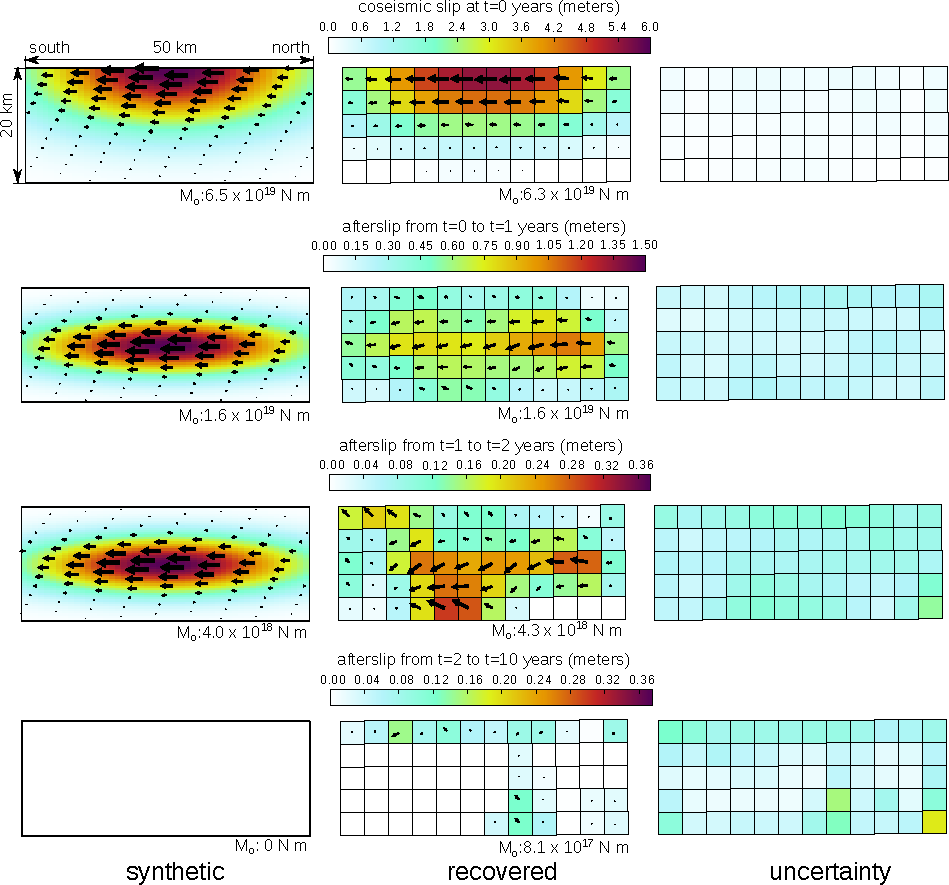
\includegraphics{ch2/figures/Fig3.pdf}
  \caption{Slip distribution imposed in both synthetic models (left),
    slip recovered for the synthetic model with Maxwell
    viscoelasticity (middle), and uncertainty in the recovered slip
    magnitude (right).  Colors indicate magnitude of slip and arrows
    indicate direction of slip (arrows pointing right indicate
    left-lateral and up is thrust).  The panels showing afterslip
    display cumulative slip over the specified time interval.  The
    slip uncertainties are the standard deviation of inferred slip
    magnitude during the specified period, which were derived from 100
    iterations of bootstrapping.}
  \label{Figure 3}
\end{figure}

\begin{figure}\label{figure4}
  \centering
  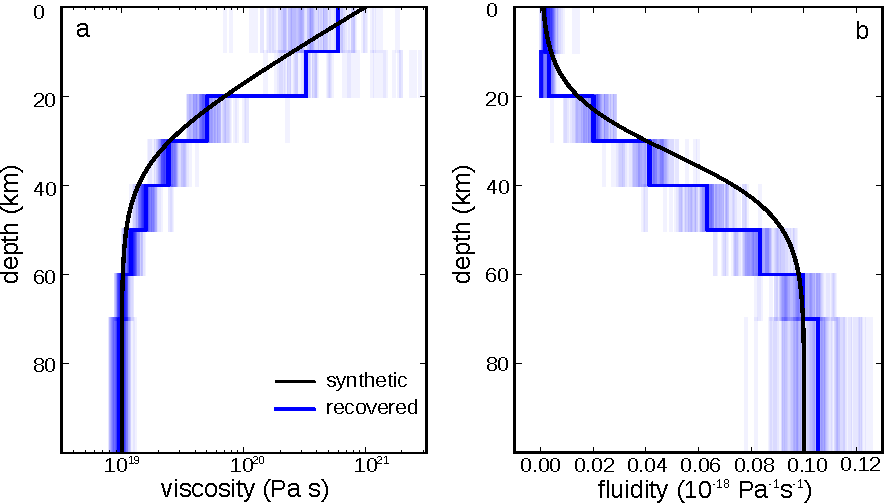
\includegraphics{ch2/figures/Fig4.pdf}
  \caption{Synthetic and recovered lithospheric viscosities (left)
    and associated fluidities (right).  Semi-transparent lines are recovered
    models found through bootstrapping and indicate the degree of
    uncertainty on the inferred viscosity structure.}
  \label{Figure 4}
\end{figure}

\begin{figure}\label{figure5}
  \centering
  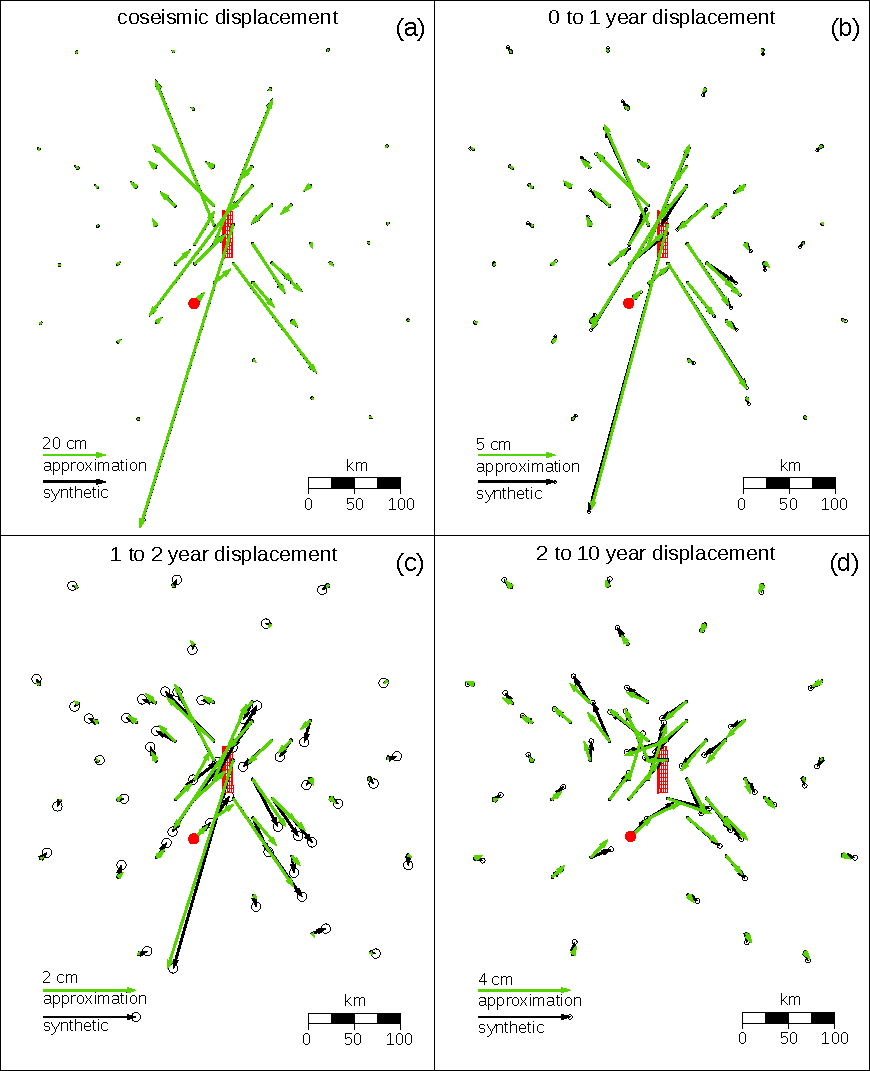
\includegraphics{ch2/figures/Fig5.pdf}
  \caption{Synthetic surface displacements (black) and best fitting
    surface displacements using eq. (\ref{Postseismic_Approximation2})
    (green).  Vertical displacements are used in the inversion but are
    not shown here. Panel (a) shows coseismic displacements
    and the remaining panels show the cumulative displacements over
    the indicated time intervals. Ellipses indicate 1 standard
    deviation uncertainty in the synthetic data. Red dot indicates the
    position of the time series shown in Fig. 6 and Fig. 9. The surface
    projection of the discretized synthetic fault is depicted in red.}
  \label{Figure 5}
\end{figure}

The lithosphere in our first synthetic model is Maxwell viscoelastic
with homogeneous Lam\'e parameters $\lambda = 32$ GPa and $\mu = 32$
GPa.  The viscosity in the lithosphere decays from $10^{21}$ Pa s
($\tau\approx1,000$ years) at the surface to $10^{19}$ Pa s
($\tau\approx10$ years) at 75 km depth (Fig. 4).  For the timescales
of this synthetic test, the uppermost lithosphere is effectively
elastic.

We use the penalty parameters chosen in Fig. 2 and our recovered model
of slip on the fault is shown in Fig. 3.  We use 100 iterations of
bootstrapping to assess how sensitive our recovered model is to the
imposed data noise.  The standard deviation of coseismic slip and
cumulative afterslip over the indicated interval is shown in the right
column of Fig. 3.  The spatial distribution and direction of inferred
coseismic slip are a good match to the synthetic coseismic slip.  The
distribution of afterslip was decently recovered but not as well as
the coseismic slip was recovered. Inferred afterslip over the first
year is smoother than the true slip due to the regularization,
although there is a high concentration of slip on the northern portion
of the fault which is consistent with the synthetic model.  We
attribute the better resolved northern portion of the fault to a
proximal surface observation point.  There are a few artifacts in the
distribution of inferred afterslip from $t=1$ to 2 years which are not
present in the synthetic model, such as slip on the deepest portion of
the fault. Our inability to recover the details of the imposed
afterslip as well as the coseismic slip could be because the data
noise is obscuring some of the postseismic signal (Fig. 5b and 5c
compared to Fig. 5a) and causing higher variability in inferred slip
models. Nevertheless, the inferred moment of both coseismic slip and
afterslip, which is proportional to slip integrated over the fault
plane, is within 10\% of the moment in the synthetic model.  Although
the spatial distribution of inferred slip may be more difficult to
recover, the slip moment seems to be consistently recovered.

The inferred slip over the last time interval, $t=2$ to 10 years, is
also consistent with the synthetic model.  The moment of slip over
this interval is $8.1\times 10^{17}$ N m, which is two orders of
magnitude smaller than the moment for the coseismic slip in the
synthetic model and is accounting for, at most, a few mm's of surface
displacement from $t=2$ to 10 years, which is on order of the data
uncertainty. We can further dismiss inferred afterslip during this
period as being negligibly small because the magnitude of inferred
slip is on order of the the uncertainty inferred from bootstrapping
(Fig. 3).  The majority of surface deformation during this time
interval (Fig. 5d) is therefore being properly attributed to
viscoelastic relaxation in the inversion results.

The inferred viscosities in each of the eight layers are shown in
Fig. 4(a).  The recovered viscosities correspond well with the
synthetic model.  The uncertainties of the recovered viscosities are
inferred using bootstrapping and we find that the strongest layers
near the surface, despite being close to the earthquake source,
have the highest uncertainties.  However, viscosities greater than
$~10^{20}$ Pa s are effectively elastic on the timescales of this
synthetic test and so a wide range of high viscosities for the upper
layers would just as adequately be able to describe the synthetic
surface displacements.  When looking at inferred values of fluidity
(Fig. 4b), we see that the uncertainties are lowest at the surface and
increase with depth, as is perhaps more intuitive.

Viscoelastic relaxation immediately below the fault and afterslip on
the fault would have similar surface manifestations, and thus it is
reasonable to explore the trade-off between these processes.  We use
the collection of models obtained through bootstrapping and compute
the correlation coefficient between the estimates of cumulative
afterslip moment over 10 years and the inferred fluidity for select
layers. Not surprisingly, the correlation coefficient is -0.16, and
-0.25 in the layer from 10 to 20 km depth and 20 to 30 km depth,
respectively, which means that higher estimates of fluidities in those
layers tend to be compensated by lower estimates of slip on the fault.
Interestingly, there is a positive correlation of 0.38 between
cumulative afterslip moment and the fluidity in the uppermost layer
containing the fault. The positive correlation is because deformation
resulting from viscoelastic relaxation in the uppermost layer
containing the fault tends to be in the opposite direction as deformation
resulting from fault slip. This means that a high fluidity in the
uppermost layer will tend to produce deformation that is balanced out by
higher amounts of slip.  It is conceivable that such a correlation
could lead to unrealistic inferences of viscosity in the near surface
and it may be necessary to assume that viscous regions containing a
fault are elastic.  There is no significant correlation between
afterslip and fluidity in layers below 30 km depth.

\subsubsection{Validation}\label{Validation}

\begin{figure}\label{figure6}
  \centering
  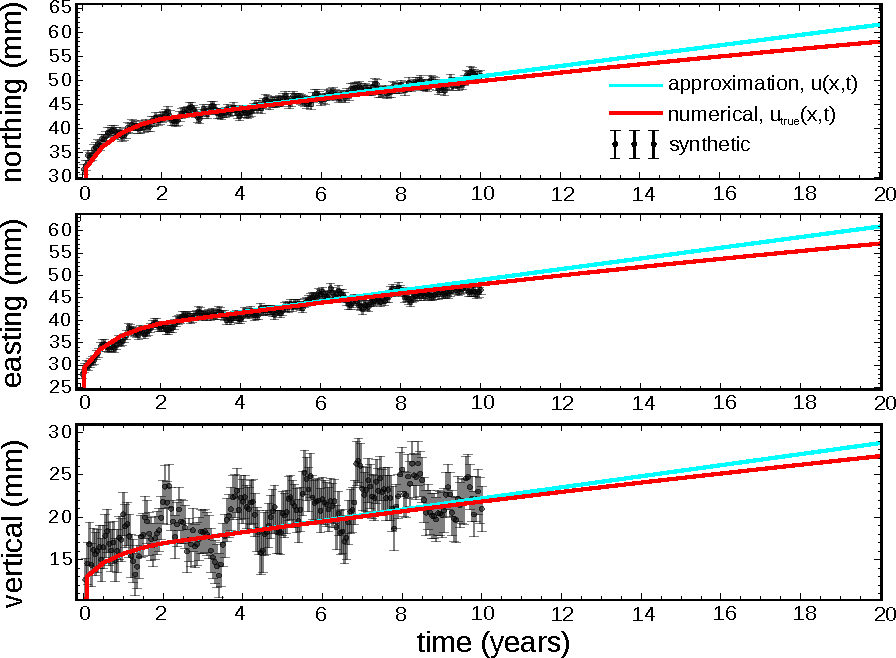
\includegraphics{ch2/figures/Fig6.pdf}
  \caption{Displacement time series for the position shown in Fig. 5
    (black), best fitting surface displacements using the
    approximation from eq. (\ref{Postseismic_Approximation2}) (green)
    and surface displacements computed with PyLith using the inferred
    slip distribution and viscosity structure (red). Coseismic displacements
    at $t=0$ are not shown.}
  \label{Figure 6}
\end{figure}

\begin{figure}\label{figure7}
  \centering
  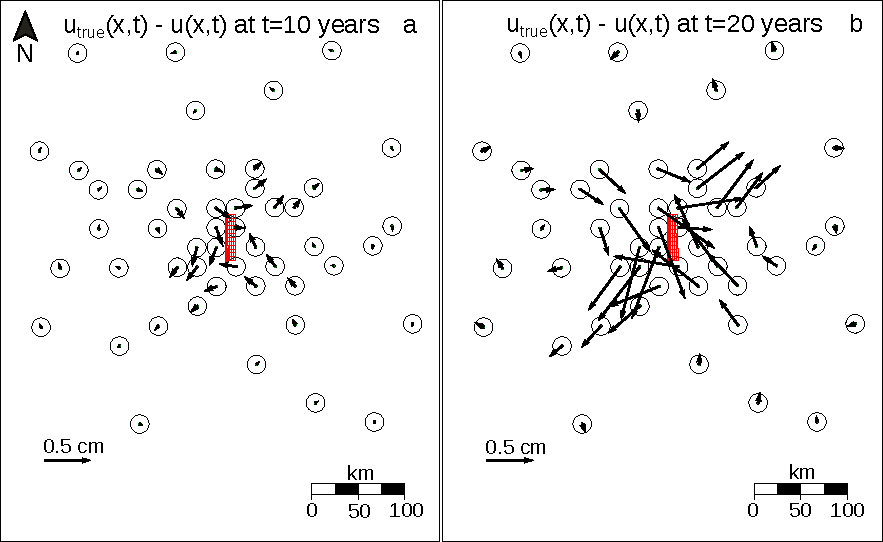
\includegraphics{ch2/figures/Fig7.pdf}
  \caption{Approximation error at $t=10$ years and $t=20$ years.
    Circles with 1 mm radius are centered at each station to compare
    the accuracy of $\vec{u}(\vec{x},t)$ to the noise in
    the synthetic data.}
  \label{Figure 7}
\end{figure}

The fact that our recovered fault slip and lithospheric viscosity are
in good agreement with the synthetic model suggests that the
approximation given by eq. (\ref{Postseismic_Approximation2}) is
accurate over the 10 years of synthetic data.  We further assess the
accuracy of eq. (\ref{Postseismic_Approximation2}) by running a
forward model with PyLith where the imposed fault slip and
lithospheric viscosity are those estimated from the synthetic data.
We then compare the displacements from the numerically computed
forward model with the displacements predicted by
eq. (\ref{Postseismic_Approximation2}).  We refer to the numerically
computed displacements as $\vec{u}_{\mathrm{true}}(\vec{x},t)$ and the
displacements predicted by the approximation as $\vec{u}(\vec{x},t)$
(Fig. 6).  We refer to the difference between
$\vec{u}_{\mathrm{true}}(\vec{x},t)$ and $\vec{u}(\vec{x},t)$ as the
approximation error (Fig. 7). At $t=10$ years the approximation error
is on order of a few mm's for each location, which is the magnitude of
the data uncertainty.  Additionally, the approximation error is small
compared to the cm's of deformation resulting from viscoelastic
relaxation, indicating that eq. (\ref{Postseismic_Approximation2}) is
indeed a fair approximation up to $t=10$ years.  At $t=20$ years the
approximation error is about one cm in magnitude for near field sites,
indicating that the approximation has broken down in the near field by
this time, while the error is still on order of a few mm's for the far
field sites.  The faster divergence for the near field sites is
consistent with the comparison we made between the approximate and
true displacements for a two-dimensional, two layered earthquake model
in Section \ref{2D2LModel} (Fig. 1).

The accuracy of eq. (\ref{Postseismic_Approximation2}) is also
demonstrated in Fig. 6, which shows $\vec{u}(\vec{x},t)$ and
$\vec{u}_{\mathrm{true}}(\vec{x},t)$ at a sample site near the fault.
The numerical solution asymptotically approaches the rate of
deformation predicted by eq. (\ref{Postseismic_Approximation2}) as
time goes to zero, demonstrating that
eq. (\ref{PostseismicInitialVelocity}) accurately describes the
initial viscoelastic response.  Additionally, the magnitude of the
difference between $\vec{u}(\vec{x},t)$ and
$\vec{u}_{\mathrm{true}}(\vec{x},t)$ is smaller than the uncertainty
of our synthetic data throughout the time series, indicating that
eq. (\ref{Postseismic_Approximation2}) is appropriate for this
synthetic test.  For this site and other near field sites, the
approximation starts to break down at about $t=10$ years. The lowest
relaxation time in our synthetic lithosphere is also about 10 years
and so the duration over which eq. (\ref{Postseismic_Approximation2})
is accurate is longer than what we found in our analysis for a
two-dimensional, two layered earthquake model in Section \ref{2D2LModel}.

\subsection{Synthetic model with Burgers viscoelasticity}\label{BurgersModel}
In the above synthetic example, we conveniently picked the length of
our displacement time series to correspond with the shortest
relaxation time in the lithosphere.  If the length of the time series
is significantly shorter than the relaxation time of the lithosphere,
then eq. (\ref{Postseismic_Approximation2}) would be an appropriate 
approximation and fault slip would be accurately recovered, although
there would not be a significant amount of deformation resulting from
viscoelastic relaxation and so inferences of viscosity would have high
uncertainty.  When the length of the time series is significantly
longer than the shortest relaxation time of the lithosphere then the
approximation would not be accurate and we would see a notable misfit
in our best fitting prediction of the data. Here we use another
synthetic test to demonstrate an iterative approach to finding the
optimal time series duration. We also use this synthetic test to
demonstrate how fluidities inferred using our inverse method can be
used to constrain the viscous properties of a non-Maxwell viscoelastic
lithosphere.

We consider a synthetic model with the same fault geometry and
prescribed slip as the synthetic model described in Section \ref{MaxModel}, but
the lithosphere now has a Burgers rheology.  A Burgers rheology can be
modeled schematically as a Maxwell spring-dashpot system connected in
series with a Kelvin spring-dashpot system. There are five rheologic
parameters needed to describe a Burgers rheology, the first Lam\'e
parameter, $\lambda$, shear moduli of the Maxwell and Kelvin elements,
$\mu_m$ and $\mu_k$, and the viscosities of the Maxwell and Kelvin
elements, $\eta_m$ and $\eta_k$.  In this synthetic test, we set
$\mu_m=\lambda=32$ GPa and $\eta_m$ equal to the viscosity structure
from the synthetic model in Section \ref{MaxModel}.  We also set $\mu_k=\mu_m$
and $\eta_k=0.1\eta_m$ so the lowest kelvin relaxation time
($\eta_k/\mu_k$) in our synthetic model is 1 year (Fig. 8).

We use the same $F_i(\vec{x})$, $G_{ij}(\vec{x})$, and $A_k(t)$,
described in Section \ref{GreensFunc} and estimate an effective
Maxwell viscosity by using 0.5, 2.0 and 5.0 years of synthetic data.
Our inverse method allows us to estimate a single value of viscosity
for each discretized region of the lithosphere and so we are unable to
recover both $\eta_k$ and $\eta_m$.  Instead, our method allows us to
estimate an effective viscosity for a Burgers viscoelastic lithosphere
during the early postseismic period.  We demonstrate in our
supplementary IPython notebook that when assuming $\mu_m$ is equal to
the shear modulus used to construct $F_i(\vec{x})$ and
$G_{ij}(\vec{x})$ then the effective fluidity inferred using our
method, $1/\eta$, is equivalent to
\begin{equation}\label{EquivalentBurgers}
\frac{1}{\eta} = \left(\frac{1}{\eta_k} + \frac{1}{\eta_m}\right).
\end{equation}

The recovered viscosities for each time series duration are shown in
Fig. 8 and we show the moment of inferred afterslip as a function of
time in Fig. 9. The synthetic and predicted displacement time series
at the observation point indicated in Fig. 5 are shown in Fig. 10.  We
are able to accurately predict the synthetic displacements (red line
in Fig. 10) and recover the fluidities expected following
eq. (\ref{EquivalentBurgers}) when using a 0.5 year time series. The
relatively few number of observations constraining the fluidity
inferences leads to large uncertainties as indicated by the
distribution of bootstrapped models.  When we use 2 years of
displacements, exceeding the minimum Kelvin relaxation time in the
synthetic model, the best fitting predicted displacements are still a
good fit to the synthetic data (green line), but it is difficult to
discern whether some of the systematic misfit is due to the inability
of eq. (\ref{Postseismic_Approximation2}) to describe the transient
displacement or because of the temporal correlation of our added
noise.  The inferences of fluidity when using 2 years of displacement
are consistently off by a factor of 0.5.  The underestimation of
fluidity is then compensated by a slight overestimation of cumulative
fault slip (Fig. 9). Although the estimated fluidities are incorrect,
the relative strength of the different layers is well recovered.  When
using 5 years of synthetic deformation, the depth dependence of
fluidity no longer resembles the true depth dependence and the
inferred moment of afterslip is appreciably higher than what was
imposed in the synthetic model. Even though additional afterslip is
describing some of the transient viscoelastic deformation, there is
still a systematic misfit in the best fitting prediction to the 5 year
time series (Fig. 10) indicating that
eq. (\ref{Postseismic_Approximation2}) is not valid for that duration
of time.  The length of the time series used for our inverse method
should be just long enough so that the best fitting predictions to the
data do not have any systematic misfit.  It is difficult to
distinguish by the fit to the data whether the model recovered using a
0.5 year time series or a 2 year time series is a better estimate of
the true model, although one can easily run a forward calculation for
each of the recovered models to see how well they predict the later
deformation.

\begin{figure}\label{figure8}
  \centering
  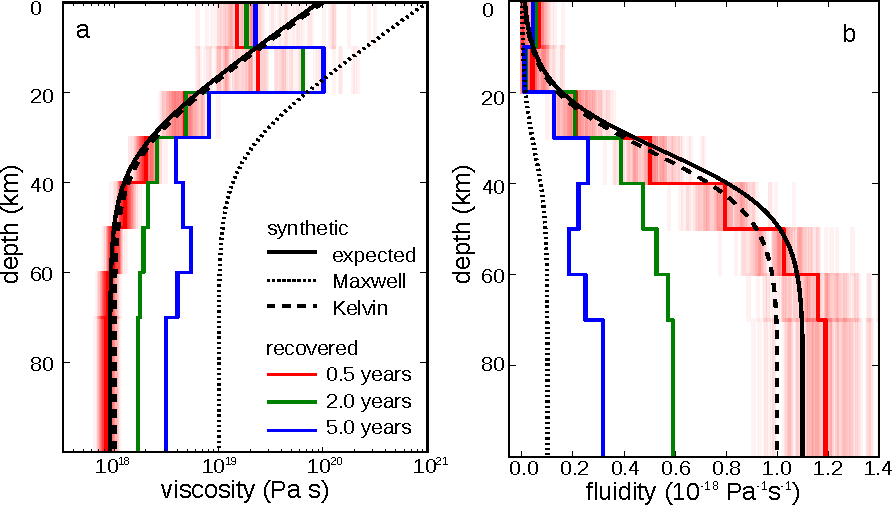
\includegraphics{ch2/figures/Fig8.pdf}
  \caption{Synthetic and recovered lithospheric viscosities (left) and
    fluidities (right) for the synthetic model with a Burgers
    rheology.  Dotted and dashed lines show the Maxwell and Kelvin
    viscosity in the synthetic model, respectively.  The solid
    black line indicates the effective viscosity from
    eq. (\ref{EquivalentBurgers}).  The red, green, and blue lines
    show the inferred viscosities and fluidities when inverting a 0.5,
    2.0, and 5.0 year long time series, respectively.  The light red
    lines are the bootstrapped fluidities and viscosities inferred
    using the 0.5 year time series.}
  \label{Figure 8}
\end{figure}

\begin{figure}\label{figure9}
  \centering
  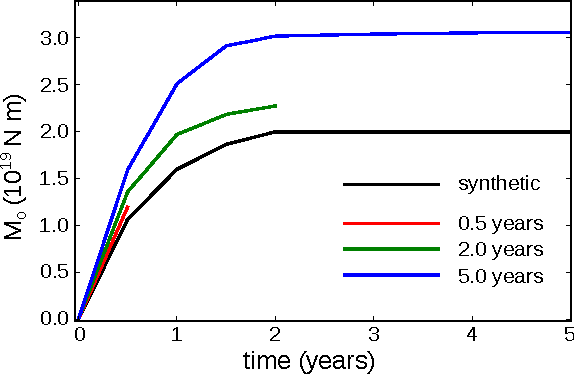
\includegraphics{ch2/figures/Fig9.pdf}
  \caption{Afterslip moment over time for the synthetic model (black) and
    the inferred afterslip moment when inverting 0.5, 2.0, and 5.0 years of
    displacements (red, green, and blue)}.
  \label{Figure 9}
\end{figure}

\begin{figure}\label{figure10}
  \centering
  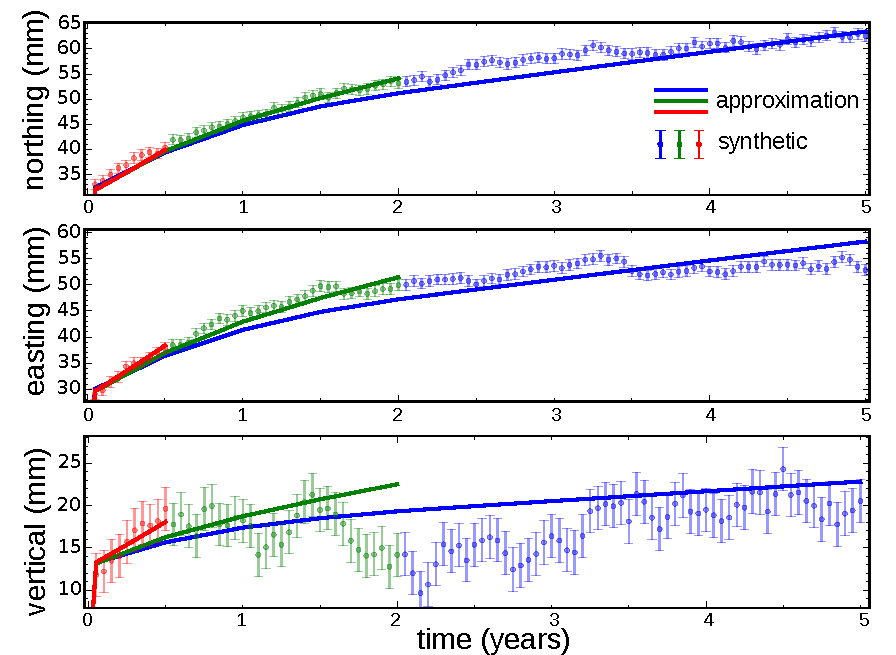
\includegraphics{ch2/figures/Fig10.pdf}
  \caption{Synthetic and predicted displacement time series with
    length 0.5, 2.0, and 5.0 years.  The time series shown is for the
    observation point indicated in Fig 5.}
  \label{Figure 10}
\end{figure}

\section{Discussion}
A fundamental assumption in our method for estimating slip and
viscosity from postseismic deformation is that the timescale of
relaxation in the weakest part of the lithosphere is at least as long
as the timescales over which postseismic deformation is observed.
This assumption allows us to approximate the surface expression of
viscous creep as a linear system with respect to lithospheric
fluidity, which greatly facilitates and expedites the inverse
problem. Since the relaxation times in a given region are generally
not well known \textit{a priori}, one must use an iterative approach as
described in Section \ref{BurgersModel} to determine the appropriate length of the time
series used in the inversion.  

We can look at previous studies to gauge the duration over which
our approximation would be accurate.  Surface deformation following large
($\geq M_w=7$) earthquakes often is characterized by transient and
rapid postseismic deformation in the first year after and earthquake
followed by steady deformation in later years
\citep[e.g.][]{Savage1997,Savage2005,Ergintav2009}.  Several studies have attributed
rapid early transient deformation following an earthquake to
afterslip, while describing the later steady deformation with viscous
relaxation in a Maxwell viscoelastic lower crust or upper mantle
\citep[e.g.][]{Perfettini2005,Johnson2009,Hearn2009,Freed2006a,Rollins2015}.  These studies have
found that lithospheric relaxation times no shorter than years or
decades are needed to describe postseismic deformation.  Indeed,
\citet{Perfettini2005} describes the trend in two years of postseismic
deformation following the 2001 $M_w=8.4$ Peru earthquake by assuming
that the lithospheric viscosity was sufficiently high that the rate of
deformation from viscoelastic creep could be considered constant,
which is the assumption that we make in formulating
eq. (\ref{Postseismic_Approximation}). If transient postseismic
deformation can be attributed to fault slip followed by steady
viscoelastic creep, then eq. (\ref{Postseismic_Approximation}) should
be able to describe displacements on the timescale of years or decades
after an earthquake.

Several studies have used rheologies containing a transient phase of
deformation to explain the early postseismic deformation.  For
example, \citet{Pollitz2003,Pollitz2005} invoked a Burgers rheology upper mantle
to explain surface displacements following the 2002 $M_w=7.9$ Denali
earthquake and the 1999 $M_w=7.1$ Hector Mine earthquake.  In both
cases the best fitting transient relaxation time was on the order of a
month and the best fitting steady-state relaxation time was on the
order of years.  Postseismic deformation following the Denali
earthquake was also successfully modeled by \citet{Freed2006b} with a
power-law rheology in the upper mantle, consistent with laboratory
studies \citep[e.g.][]{Kirby1987}.  The power-law rheology was able to
reproduce the observed transient surface deformation because the high
stresses in the earthquake decreased the effective viscosity of the
upper mantle to $\sim10^{17}$ Pa s resulting in fast surface
deformation.  As stresses from the earthquake relaxed, the effective
viscosity increased and the predicted surface deformation became
steadier. Based on the success of \citet{Pollitz2003,Pollitz2005} and
\citet{Freed2006b}, one may dismiss our method as being unrealistic
because we assume that the lithosphere is Maxwell viscoelastic.
However, our method does not necessarily preclude the possibility of a
Burgers rheology, as demonstrated in Section \ref{BurgersModel}, or a
stress-nonlinear viscosity.  As long as stresses in the lithosphere
remain roughly equal to the the stresses transferred elastically
through fault slip, then a viscosity structure inferred using our
method could be interpreted as the effective viscosity in a transient
viscoelastic or power-law rheology.  One could also use
eq. (\ref{EquivalentBurgers}) to constrain the rheologic properties
for a Burgers rheology.  If the commonly observed early transient
postseismic deformation truly is the result of viscous relaxation in
the lithosphere rather than afterslip, then the results from
\citet{Pollitz2003,Pollitz2005} and \citet{Freed2006b} suggest that the time interval
over which eq. (\ref{Postseismic_Approximation}) is appropriate is on
order of a month after an earthquake.  In such case, our method can be
used to get an initial estimate of lithospheric viscosity, while
unused portion of the displacement time series could be incorporated
in a gradient based nonlinear inverse method where the forward problem
is computed numerically rather than with
eq. (\ref{Postseismic_Approximation}).

Postseismic transient deformation could also be the result of creep in
a weak ductile shear zone which is embedded in a stronger viscoelastic
lithosphere \citep[e.g.][]{Hetland2014}. Sufficiently localized creep in a
shear zone can be modeled as slip on a down-dip extension of the
ruptured fault \citep[e.g.][]{Hearn2002,Kenner2003,Johnson2004} because the two
processes are kinematically indistinguishable.  Likewise,
\citet{Freed2006b} noted that deep fault slip could serve as a proxy for
distributed viscous relaxation in a weak lower crust when only
considering horizontal displacements. The applicability of our method
should therefore be unaffected by localized viscous deformation with
the understanding that inferences of fault slip could be absorbing
that deformation.


\section{Conclusion}
We present a method to invert coseismic and postseismic deformation to
simultaneously estimate a time dependent distribution of fault slip
and an arbitrarily discretized viscosity structure of the lithosphere.
We take advantage of an approximation for early postseismic
deformation resulting from fault slip and viscoelastic relaxation.
This approximation is computationally efficient which allows us to
rapidly search a high dimensional model space and make higher
resolution estimates of effective lithospheric viscosity than what can
feasibly be done with the commonly used grid search methods. Our
method is applicable for as long as this approximation is appropriate,
that is, for as long as stresses resulting from coseismic slip and
afterslip have not significantly decayed due to viscoelastic
relaxation.  Based on inferences of lithospheric viscosity from other
studies, we estimate that our method could be used for postseismic
deformation ranging from months to years after an earthquake.
Despite our methods application to a limited portion of the
postseismic period, we demonstrate that our method is capable of
robustly recovering the mechanisms driving postseismic deformation.


\bibliographystyle{agu04}
\bibliography{refs}

\newappendix{Appendix 2A: Inverse Laplace transform through series expansion}
Let $f(t)$ be analytic at $t=0$ and let there
  be a real valued $M$, and $C$ such that
\begin{equation}\label{constraints}
  \left|f^{(n)}(t)\right| < Ce^{Mt}\quad \forall t\geq 0\text{ and }\forall n\in\{0,1,2,\dots\},
\end{equation}
where $f^{(n)}(t)$ denotes the $n^{th}$ derivative of $f(t)$.  We
define the Laplace transform of $f(t)$ as
\begin{equation}
  \mathcal{L}[f(t)] := \hat{f}(s) := \int_{0}^\infty f(t)e^{-st}dt
\end{equation}
and we restrict our attention to $s\in\mathbb{R}$.  The constraints on
$f^{(n)}(t)$ from eq. (\ref{constraints}) ensure that
\begin{equation}\label{Property2}
  \lim_{s \to \infty}\mathcal{L}[f^{(n)}(t)] = 0.
\end{equation}
It can be shown using integration by parts that
\begin{equation}\label{Property1}
  \mathcal{L}[f^{(n)}(t)] = s^n\hat{f}(s) - \sum_{m=1}^ns^{m-1}f^{(n-m)}(0)
  \quad \forall s>M.
\end{equation}
Substituting eq. (\ref{Property1}) into eq. (\ref{Property2}) and then
rearranging the terms gives us a recursive formula for $f^{(n)}(0)$ in
terms of $\hat{f}(s)$:
\begin{equation}\label{NthDeriv}
  f^{(n)}(0) = \lim_{s \to \infty} s^{n + 1}\hat{f}(s) -
               \sum_{m=1}^{n} s^{m}f^{(n-m)}(0),
\end{equation}
where the base case, $n=0$, is the initial value theorem:
\begin{equation}\label{NthDerivBase}
  f(0) = \lim_{s \to \infty} s\hat{f}(s).
\end{equation}
Since we request $f(t)$ to be analytic at $t=0$, we can construct a
Taylor series expansion of $f(t)$ such that
\begin{equation}\label{TaylorSeries}
  f(t) = \sum_{n=0}^\infty\frac{f^{(n)}(0)}{n!}t^n
\end{equation}
for all values of $t$ within some neighborhood of $t=0$. We find the
inverse Laplace transform of $\hat{f}(s)$ by combining
eq. (\ref{TaylorSeries}) with eqs. (\ref{NthDeriv}) and
(\ref{NthDerivBase}) so that $f(t)$ is expressed in terms of
$\hat{f}(s)$.


\newappendix{Appendix 2B: Postseismic approximation for a two-dimensional earthquake model with a depth dependent viscosity}
We seek to find an approximation for early postseismic deformation in
a two-dimensional, strike-slip earthquake model with an arbitrary
depth-dependent viscosity below the fault locking depth, $D$.  We
first find the initial rate of surface deformation following a unit of
slip in a lithosphere that is elastic except for a viscoelastic layer
which is at depth $z$ and with thickness $\Delta z$. This is found by
making the substitutions $H_1 \to z$, $H_2 \to \Delta z$, $\eta_1 \to
\infty$, $\eta_3 \to \infty$, and $\eta_2 \to \eta$ in
eq. (\ref{ThreeLayerViscousResponse}), which gives us
\begin{equation}
  \frac{\partial}{\partial t}u_1(x,t)\big|_{t=0} = 
  \frac{1}{\eta}(W(z+\Delta z) - W(z)),
\end{equation}
where
\begin{equation}
  W(z) = \frac{\mu}{2\pi}\left(\tan^{-1}\left(\frac{2z-D}{x}\right) -
  \tan^{-1}\left(\frac{2z+D}{x}\right)\right).
\end{equation}
From eq. (\ref{PostseismicInitialVelocity}) we know that the initial
rate of surface deformation for a lithosphere composed of $N$ discrete
layers, each with viscosity $\eta_i$, at depth $z_i$, and having
thickness $\Delta z$, is then
\begin{equation}
  \frac{\partial}{\partial t}u_N(x,t)\big|_{t=0} = \sum_i^N
  \frac{1}{\eta_i}(W(z_i + \Delta z) - W(z_i)).
\end{equation}
The initial rate of surface deformation for a viscosity structure
given by $\eta(z)$ is found by taking the limit as $\Delta z \to 0$
and $N \to \infty$:
\begin{align}\label{ArbitraryViscousResponse}
 \frac{\partial}{\partial t}u(x,t)\big|_{t=0} &= \int_D^\infty
 \frac{1}{\eta(z)}\frac{\partial}{\partial z} W(z) dz\\
 &= \int_D^{\infty}\frac{\mu}{2\pi\eta(z)}\left(\frac{2x}{x^2 + \left(D + 2z\right)^2} -
                     \frac{2x}{x^2 + \left(2z - D\right)^2}\right) dz.
\end{align}
Finally, we add the elastic component of deformation and integrate
eq. (B.5) with the fault slip history to obtain
an approximation for early postseismic deformation:
\begin{equation}
u(x,t) \approx \frac{b(t)}{\pi}\tan^{-1}(\frac{D}{x}) + 
               \int_o^t\int_D^\infty \frac{\mu b(\theta)}{2\pi\eta(z)}
                                    \left(\frac{2x}{x^2 + \left(D + 2z\right)^2} - 
                                    \frac{2x}{x^2 + \left(2z - D\right)^2}\right)
                                    dz d\theta.
\end{equation}
